\documentclass[11pt,letterpaper]{article}

\newenvironment{proof}{\noindent{\bf Proof:}}{\qed\bigskip}

\newtheorem{theorem}{Theorem}
\newtheorem{corollary}{Corollary}
\newtheorem{lemma}{Lemma} 
\newtheorem{claim}{Claim}
\newtheorem{fact}{Fact}
\newtheorem{definition}{Definition}
\newtheorem{assumption}{Assumption}
\newtheorem{observation}{Observation}
\newtheorem{example}{Example}
\newcommand{\qed}{\rule{7pt}{7pt}}

\newcommand{\solution}[4]{
\thispagestyle{plain} 
\newpage
\setcounter{page}{1}
\noindent
\begin{center}
\framebox{ \vbox{
\vspace{4mm}
\vspace{0.2in} 
{\centering \large\mbox{#3}}\\
\vspace{0.1in}
{#1 \hfill {Date: #2}}
}}
\end{center}
\markright{#1}
}

\newenvironment{algorithm}
{\begin{center}
\begin{tabular}{|l|}
\hline
\begin{minipage}{1in}
\begin{tabbing}
\quad\=\qquad\=\qquad\=\qquad\=\qquad\=\qquad\=\qquad\=\kill}
{\end{tabbing}
\end{minipage} \\
\hline
\end{tabular}
\end{center}}

\def\Comment#1{\textsf{\textsl{$\langle\!\langle$#1\/$\rangle\!\rangle$}}}



\usepackage{graphicx, amssymb, amsmath, listings, float, mathtools}
\usepackage{color, url}
\lstset{language = Python}
\lstset{breaklines}
\lstset{extendedchars=false}

\oddsidemargin 0in
\evensidemargin 0in
\textwidth 6.5in
\topmargin -0.6in
\textheight 9.0in

\begin{document}

\solution{\large Jifu Zhao}{\large 09/29/2016}{\bf \Large ECE 544NA \hspace{0.5cm} 
		Fall 2016 \hspace{0.5cm} Assignment 2}

\section*{\Large I. Pencil-and-Paper}
\begin{description}
%%%%%%%%%%%%%%%%%%%%%%%%%%%%%%%%%%%%%%%%%%%%%%%%%%%%%%%%%%%%%%%%%%%%%%%%%%%%%%%%%%%%%%%%%
% Problem 1
\item{\bf \large 1. } Derivative of Softmax \\
Recall the softmax function:
\begin{equation}
	\vec{y}[k] = \frac{e^{\vec{z}[k]}}{\sum_{l=1}^C e^{\vec{z}[l]}}
\end{equation}

So, consider two cases, j = k and j != k. 

When j = k:
\begin{equation}
	\frac{\partial \vec{y}[k]}{\partial \vec{z}[j]} 
		= - \frac{e^{\vec{z}[k]} \cdot \sum_{l=1}^C e^{\vec{z}[l]} - e^{\vec{z}[k]} \cdot e^{\vec{z}[k]}} 
				{(\sum_{l=1}^C e^{\vec{z}[l]})^2}
		= \vec{y}[k] - \vec{y}[k] \cdot \vec{y}[k]
\end{equation}

When j != k:
\begin{equation}
	\frac{\partial \vec{y}[k]}{\partial \vec{z}[j]} 
		= - \frac{e^{\vec{z}[k]} \cdot e^{\vec{z}[j]}} 
				{(\sum_{l=1}^C e^{\vec{z}[l]})^2}
		= - \vec{y}[k] \cdot \vec{y}[j]
\end{equation}

So, we can conclude that:
\begin{equation}
	\frac{\partial \vec{y}[k]}{\partial \vec{z}[j]} = 
	\begin{cases}
		- \vec{y}[k] \cdot \vec{y}[j]				& \quad \text{if } k != j \\
		\vec{y}[k] - \vec{y}[k] \cdot \vec{y}[k]	& \quad \text{if } k = j \\
	\end{cases}
\end{equation}


%%%%%%%%%%%%%%%%%%%%%%%%%%%%%%%%%%%%%%%%%%%%%%%%%%%%%%%%%%%%%%%%%%%%%%%%%%%%%%%%%%%%%%%%%
% Problem 2
\item{\bf \large 2. } Negative Log Likelihood loss for Multi-Class. \\
Recall the negative log likelihood: 
\begin{equation}
	L = - \sum_i^N \sum_k^K {\bf 1}[y_i = k] \cdot log(\hat{\vec{y}}_i[k])
\end{equation}

In this way, we have:
\begin{equation}
	\frac{\partial L}{\partial \hat{\vec{y}}_i[j]} 
	= - {\bf 1}[y_i = k] \cdot \frac{\partial log(\hat{\vec{y}}_i[j])}{\partial \hat{\vec{y}}_i[j]}
	= - \frac{{\bf 1}[y_i = j]}{\hat{\vec{y}}_i[j]}
\end{equation}


%%%%%%%%%%%%%%%%%%%%%%%%%%%%%%%%%%%%%%%%%%%%%%%%%%%%%%%%%%%%%%%%%%%%%%%%%%%%%%%%%%%%%%%%%
% Problem 3
\item{\bf \large 3. } Avg-pooling (1D) \\
Recall Avg-pooling (1D) operation with window size W: 
\begin{equation}
	\vec{y}[i] = \frac{1}{W} \sum_{j=0}^W \vec{x}[i + j]
\end{equation}

Then, we have:
\begin{equation}
	\frac{\partial \vec{y}[i]}{\partial \vec{x}[j]} = 
		\begin{cases}
			- \frac{1}{W}	& \quad \text{if } i \leq j \leq i + W \\
			0				& \quad \text{otherwise} \\
		\end{cases}
\end{equation}

%%%%%%%%%%%%%%%%%%%%%%%%%%%%%%%%%%%%%%%%%%%%%%%%%%%%%%%%%%%%%%%%%%%%%%%%%%%%%%%%%%%%%%%%%
% Problem 4
\item{\bf \large 4. } Max-pooling (1D) \\
Recall Max-pooling (1D) operation with window size W: 
\begin{equation}
	\vec{y}[i] = \max_{j=0}^W \vec{x}[i + j]
\end{equation}

Then, we have:
\begin{equation}
	\frac{\partial \vec{y}[i]}{\partial \vec{x}[j]} = 
		\begin{cases}
			1	& 	\quad \text{if } \max_{k=0}^W \vec{x}[i + k] = \vec{x}[j] \\
			0	& 	\quad \text{otherwise} \\
		\end{cases}
\end{equation}


%%%%%%%%%%%%%%%%%%%%%%%%%%%%%%%%%%%%%%%%%%%%%%%%%%%%%%%%%%%%%%%%%%%%%%%%%%%%%%%%%%%%%%%%%
% Problem 5
\item{\bf \large 5. } Convolutional layer (1D)\\
Recall Convolution (1D) operation, assume $\vec{w}$ is length 3, and zero index at the center:
\begin{equation}
	\vec{y}[i] = (\vec{w} \ast \vec{x})[i] = \sum_{j=-1}^1 \vec{x}[i-j] \cdot \vec{x}[j]
\end{equation} 

From above equation, we have:
\begin{equation}
	\frac{\vec{y}[i]}{\vec{x}[j]} =
	\begin{cases}
			\vec{w}[i-j]	& 	\quad \text{if } i-1 \leq j \leq i+1 \\
			0	& 	\quad \text{otherwise} \\
		\end{cases}
\end{equation}

\begin{equation}
	\frac{\vec{y}[i]}{\vec{w}[j]} =
	\begin{cases}
			\vec{x}[i-j]	& 	\quad \text{if } j = -1 or 0 or 1 \\
			0				& 	\quad \text{otherwise} \\
		\end{cases}
\end{equation}
\end{description}

\newpage
\section*{\Large II. Code-from-Scratch}

\subsection*{\large 1. Methods}

\begin{figure}[H]
\centering
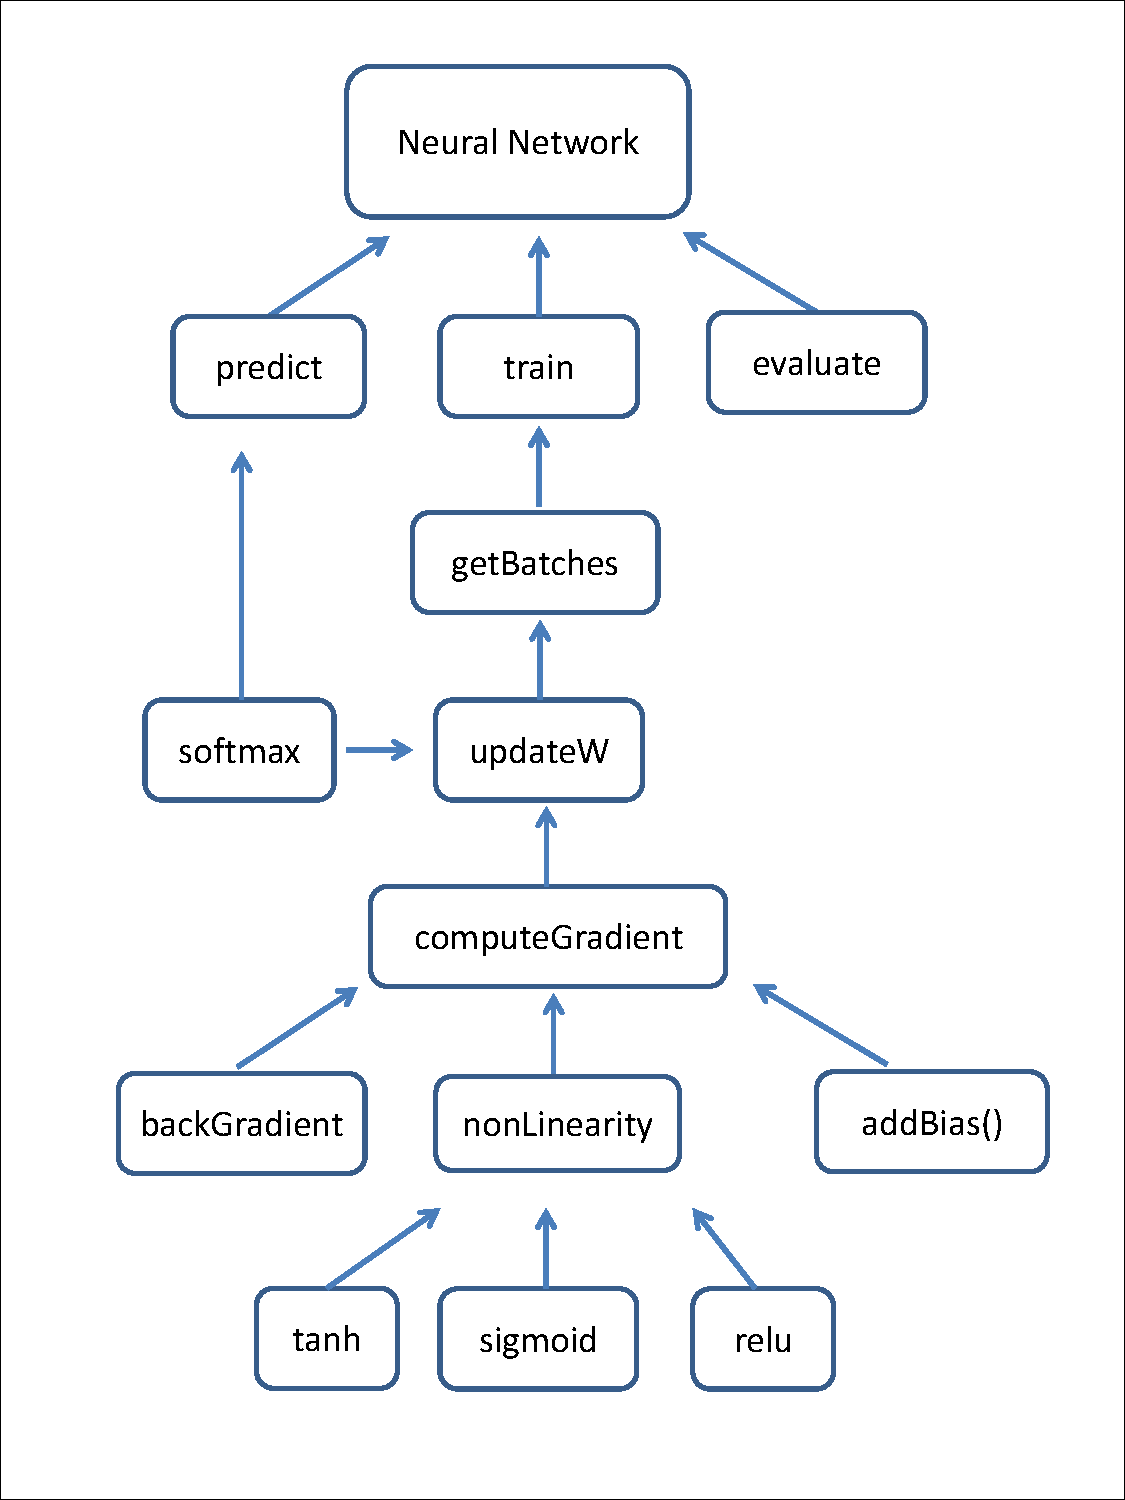
\includegraphics[width=0.6\textwidth]{./figures/ECE544hw2.pdf}\
\caption{\label{fig:structure} Algorithm Structure}
\end{figure}


\subsection*{\large 2. Results}

\begin{table}[H]
	\centering
	\caption{Comparison of training accuracy}
	\label{table:trainAcc}	
	\begin{tabular}{c | c | c | c }
		\hline \hline
		Hidden Nodes/Function	&	ReLU	& 	Sigmoid		&	 Tanh 	\\[0.1cm]
		\hline
		10						&	66.42\%	&	57.25\%		&	 63.16\% \\[0.1cm]
		20						&	87.94\%	&	76.72\%		&	 59.21\% \\[0.1cm]
		30						&	60.71\%	&	78.08\%		&	 75.35\% \\[0.1cm]
		40						&	56.84\%	&	83.69\%		&	 77.91\% \\[0.1cm]
		50						&	69.90\%	&	83.67\%		&	 79.72\% \\[0.1cm]
		\hline	
	\end{tabular}
\end{table}

\begin{table}[H]
	\centering
	\caption{Comparison of test accuracy}
	\label{table:testAcc}	
	\begin{tabular}{c | c | c | c }
		\hline \hline
		Hidden Nodes/Function	&	ReLU	& 	Sigmoid		&	 Tanh 	\\[0.1cm]
		\hline
		10						&	39.38\%	&	43.01\%		&	 41.03\% \\[0.1cm]
		20						&	43.34\%	&	46.09\%		&	 44.44\% \\[0.1cm]
		30						&	43.23\%	&	44.44\%		&	 44.11\% \\[0.1cm]
		40						&	35.42\%	&	45.10\%		&	 46.09\% \\[0.1cm]
		50						&	40.70\%	&	46.31\%		&	 43.01\% \\[0.1cm]
		\hline	
	\end{tabular}
\end{table}


\begin{table}[H]
	\centering
	\caption{Average time for one iteration (in seconds)}
	\label{table:time}	
	\begin{tabular}{c | c | c | c }
		\hline \hline
		Hidden Nodes/Function	&	ReLU	& 	Sigmoid		&	 Tanh 	\\[0.1cm]
		\hline
		10						&	0.00067	&	0.00309		&	 0.00509 \\[0.1cm]
		20						&	0.00073	&	0.00330		&	 0.00535 \\[0.1cm]
		30						&	0.00082	&	0.00352		&	 0.00555 \\[0.1cm]
		40						&	0.00092	&	0.00366		&	 0.00582 \\[0.1cm]
		50						&	0.00105	&	0.00383		&	 0.00614 \\[0.1cm]
		\hline	
	\end{tabular}
\end{table}


\begin{figure}[H]
\centering
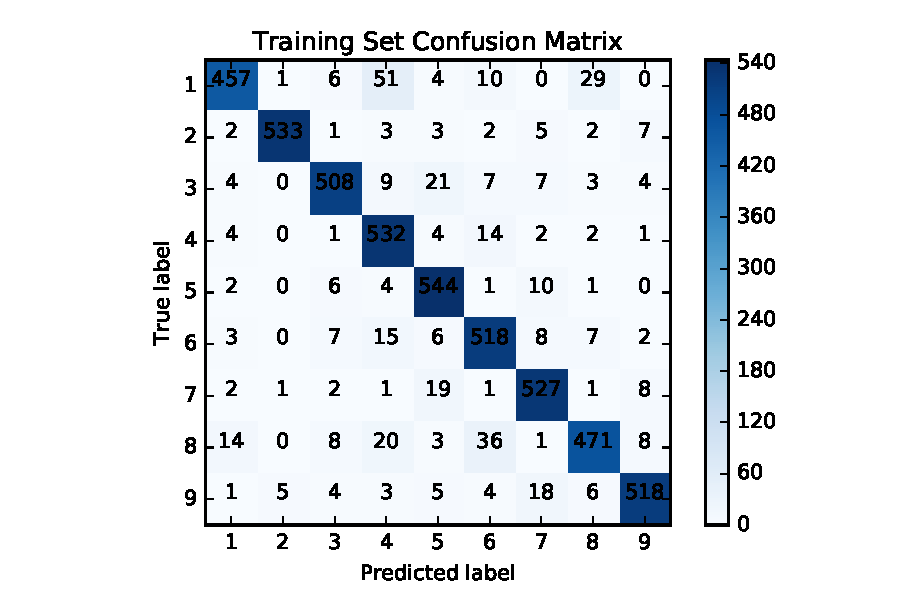
\includegraphics[width=1.0\textwidth]{./figures/trainMatrix.pdf}\
\caption{\label{fig:trainMatrix} Training Set Confusion Matrix}
\end{figure}


\begin{figure}[H]
\centering
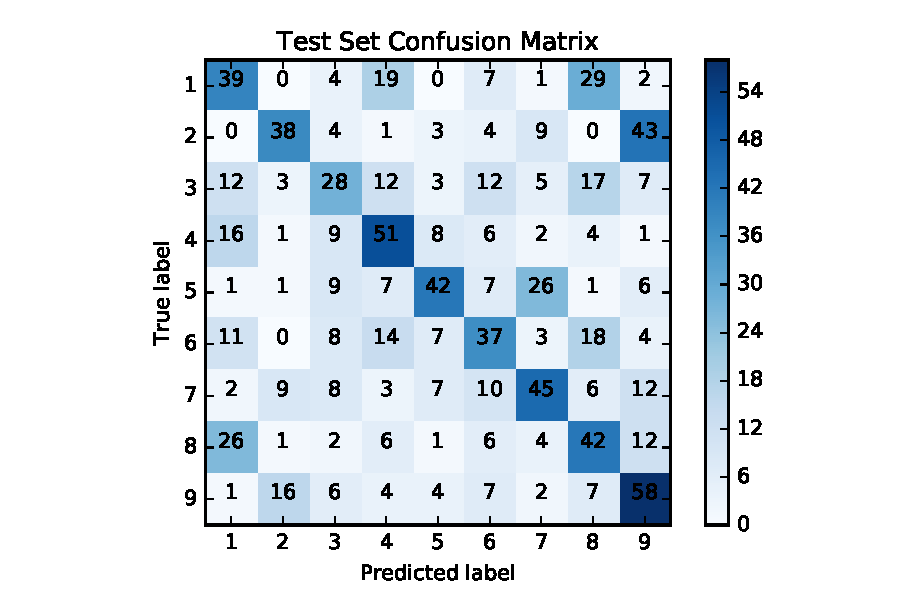
\includegraphics[width=1.0\textwidth]{./figures/testMatrix.pdf}\
\caption{\label{fig:testMatrix} Test Set Confusion Matrix}
\end{figure}


\newpage
\section*{\Large III. TensorFlow}

\subsection*{\large 1. Methods}

\subsection*{\large 2. Results}

%\begin{figure}[H]
%\centering
%\includegraphics[width=0.8\textwidth]{./figures/TDNNtrainMatrix.pdf}\
%\caption{\label{fig:TDNNtrainMatrix} Training Set Confusion Matrix for TDNN model}
%\end{figure}
%
%
%\begin{figure}[H]
%\centering
%\includegraphics[width=0.8\textwidth]{./figures/TDNNtestMatrix.pdf}\
%\caption{\label{fig:TDNNtestMatrix} Test Set Confusion Matrix for TDNN model}
%\end{figure}



%\begin{figure}[H]
%\centering
%\includegraphics[width=0.8\textwidth]{./figures/BESTtrainMatrix.pdf}\
%\caption{\label{fig:BESTtrainMatrix} Training Set Confusion Matrix for best model}
%\end{figure}
%
%
%\begin{figure}[H]
%\centering
%\includegraphics[width=0.8\textwidth]{./figures/BESTtestMatrix.pdf}\
%\caption{\label{fig:BESTtestMatrix} Test Set Confusion Matrix for best model}
%\end{figure}


\clearpage

%\bibliographystyle{plain}
%\bibliographystyle{unsrt}
%\bibliography{reference.bib}

\end{document}

